After testing our VV solver for the two-body case, 
we extend our program to solve the Earth-Sun-Jupiter (three-body) system and then the whole solar system. 
This extension is done easily thanks to object-oriented programming. 
Fig. \ref{fig:threebody} shows the orbits of the Earth-Sun-Jupiter system with different Jupiter mass. 
The total time is 100 years. 
In Fig. \ref{fig:leftthree}, when we fix the position of the Sun and set Jupiter mass as $1\times$ and $10\times$ the actual Jupiter mass, 
the orbit of the Earth is still a quite good circle, and we can hardly see any difference between $1\times$ and $10\times$ cases. 
When we do not fix the position of the Sun and fix the center of mass at origin, 
the orbit of the Earth hardly changes. 
So in the above three cases the influence of Jupiter on Earth can be treated perturbatively. 
But when we increase the mass of Jupiter to $1000\times$ (Fig. \ref{fig:rightthree}), 
the Earth flies away and the system seems to be unstable. 
In this case the Sun and Jupiter have almost the same mass, 
and thus the Sun should not be fixed and the whole system is an unstable "binary stars + one planet" system. 
\begin{figure}[tb]
	\begin{subfigure}[tb]{0.5\textwidth}
		\centering
		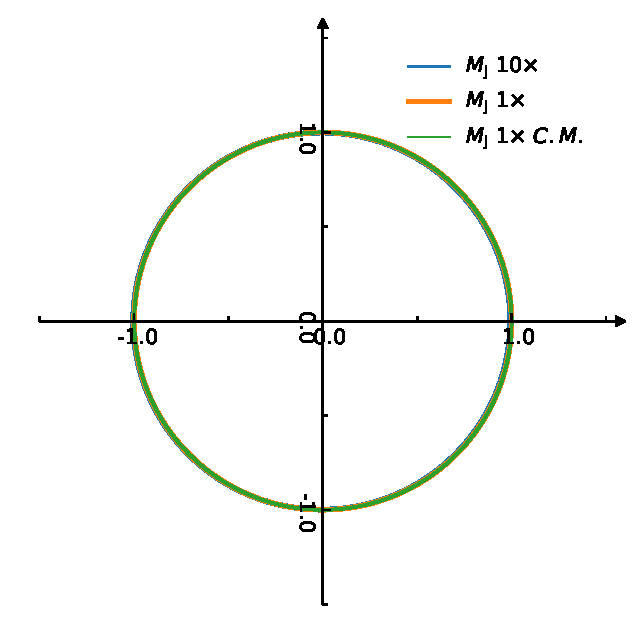
\includegraphics[width=0.7\textwidth]{SEJ_CM.eps}
		\caption{}
		\label{fig:leftthree}
	\end{subfigure}
	~
	\begin{subfigure}[tb]{0.5\textwidth}
		\centering
		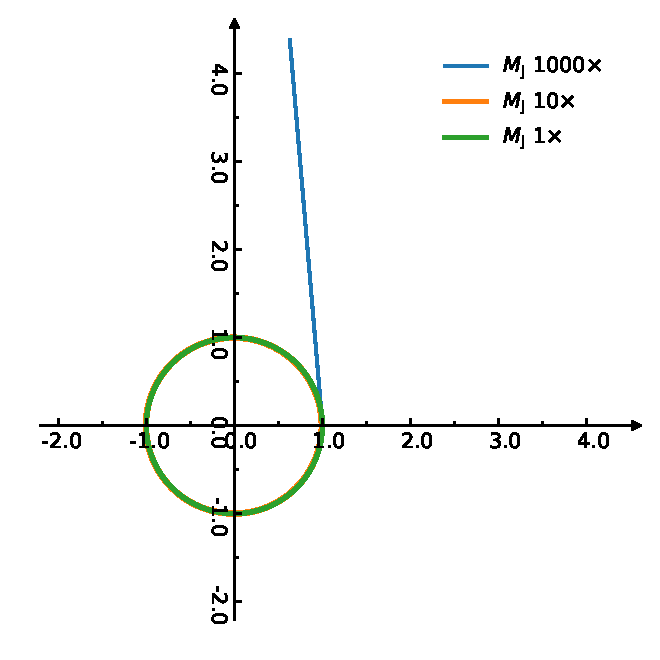
\includegraphics[width=0.7\textwidth]{SEJ.eps}
		\caption{}
		\label{fig:rightthree}
	\end{subfigure}
	\caption{Orbit of the Earth in the Earth-Sun-Jupiter system with different Jupiter mass. 
	C.M. represents that the Sun is not fixed and the center of mass is at origin. 
	Total time is 100 years. The unit of coordinate is AU. }
	\label{fig:threebody}
\end{figure}
\par
After confirming the stability of VV method in the three-body system, 
we simulate the whole solar system using the positions and velocities of the Sun and eight planets 
at A.D. 2018-Apr-02 00:00:00.0000 TDB \cite{NASAdata} as the initial condition. 
Fig. \ref{fig:solarsystem} shows the orbits of the Sun and all the planets. 
The total time is 200 years, longer than the period of Neptune. 
Also, the center of mass is fixed at origin. 
In our simulation, motions in $x$, $y$ and $z$ directions are all calculated. 
But as the motion in $z$ direction is not significant compared to that in $x-y$ plane, 
we only plot the projection of orbits in $x-y$ plane. 
From Fig. \ref{fig:solarsystem}, we can see that the whole system is stable. 
Because of the large mass of the Sun, its orbit can hardly be seen in the figure. 
The orbit of Mercury is not a closed oval because of the impact from otter planets. 
The orbits of other planets are almost closed, and their relative eccentricities agree with the observation. 
\begin{figure}[bt]
	\begin{subfigure}[tb]{0.5\textwidth}
		\centering
		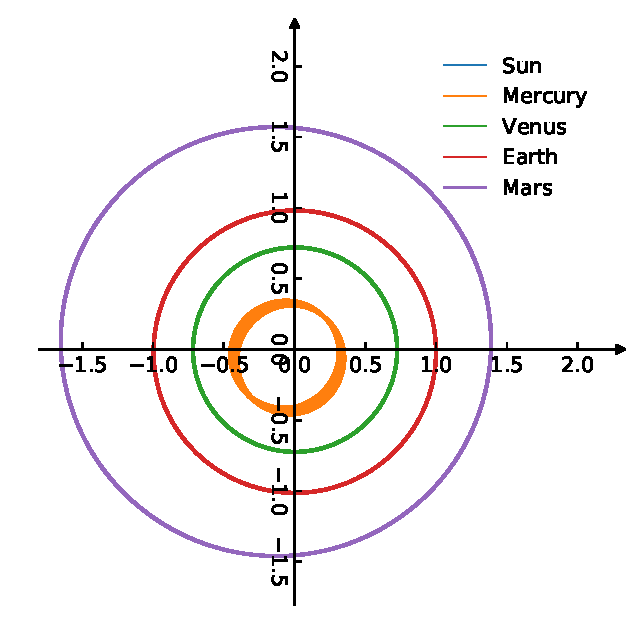
\includegraphics[width=0.7\textwidth]{solar1.eps}
		\caption{The Sun and inner planets. }
		\label{fig:solarinner}
	\end{subfigure}
	~
	\begin{subfigure}[tb]{0.5\textwidth}
		\centering
		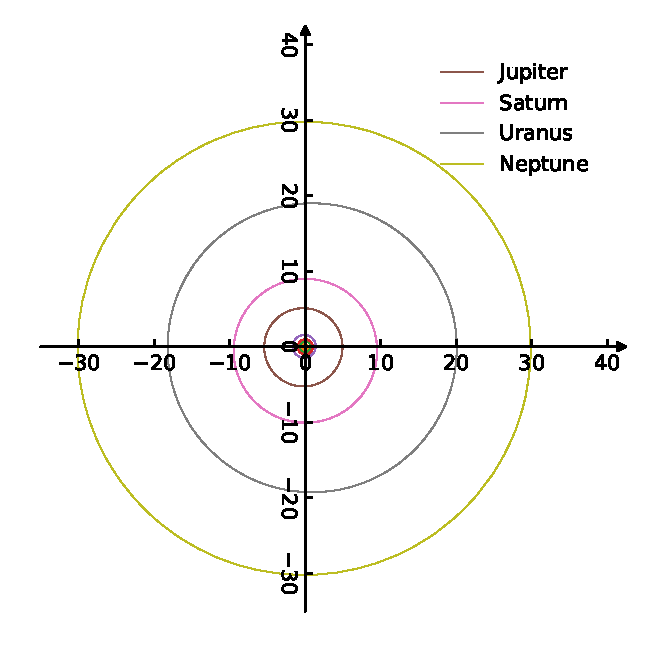
\includegraphics[width=0.7\textwidth]{solar2.eps}
		\caption{Outer planets. }
		\label{fig:solarouter}
	\end{subfigure}
	\caption{Orbits of the Sun and all the planets. The center of mass is fixed at origin. 
		Total time is 200 years. The unit of coordinates is AU. }
	\label{fig:solarsystem}
\end{figure}